\chapter{Chapter 4 - The Freemium Model in Indoor Maps Survey - Results}
This chapter aims to present the results of the survey to the reader, and the questions and the respective responses will be presented here. The respective questions have been grouped according to their nature of inquiry.
A total of 14 respondents of the survey submitted answers, and in total 60 institutions were contacted. This leads to a response rate of $23.3\%$. 
\section{Respondents}
Several respondents indicated that they were some sort of leading figure; headmasters at HEIs and building- and operations managers. Given the anonymity of the survey, only four respondents chose to specify who they represented and their current position. In the case of hospitals, the invitation letter sent through e-mail was sent to all eligible receivers which meant that personnel that would not be qualified to answer the survey, received the letter. This was unintentional from the surveyor's point of view and was further clarified in the proceeding invitation letters.

\begin{table}[htbp]
\centering
\begin{tabular}{|c|p{2cm}|p{0.8\linewidth}|}
\hline
\textbf{Keyword} & \textbf{Question Group} & \textbf{Question asked}                                                                                                                                                                                                                                         \\ \hline
Q1               & 1                       & \pbox{10cm}{At the moment, how can one locate and/or \\ navigate to a desired indoor location?}                                                                                                                                                                                 \\ \hline
Q2               & 1                       & \pbox{10cm}Are you currently using an indoor map system?                                                                                                                                                                                                                   \\ \hline
Q3               & 2                       & \pbox{10cm}{If currently not using an indoor map system, \\are you considering using an indoor map system?}                                                                                                                                               \\ \hline
Q4               & 2                       & \pbox{10cm}{Alternatively, how much would you be willing to pay for \\such a system?}                                                                                                                                                                                          \\ \hline
Q5               & 2                       & \pbox{10cm}{If the system is free in its basic form, how would such \\a proposition be met?}                                                                                                                                                                                   \\ \hline
Q6               & 2                       & \pbox{10cm}{Would additional, value-adding, paid services on top of a free, \\basic service be of interest?}                                                                                                                                                                     \\ \hline
Q7               & 3                       & \pbox{10cm}{If such a system is not wanted in general terms, \\which underlying factors decides this?}                                                                                                                                                                         \\ \hline
Q8               & 4                       & \begin{tabular}[c]{@{}l@{}}Please rank the following services: "Navigation and indoor \\pathfinding", "integration with SMS and own apps", \\ "integration with timetables", "automatic updating of maps"\\ and "integration of maps into own systems"\end{tabular} \\ \hline
Q9               & 5                       & \pbox{10cm}{If you already have an indoor map system, \\would there be more or less interest in a free system \\with potential value-added services?}                                                                                                                            \\ \hline
\end{tabular}
\caption{Questions asked in the Freemium Model in Indoor Maps Survey}
\label{table:questions}
\end{table}



\section{Current Indoor Mapping Situation - Group 1}
Figure \ref{table:questions} presents all questions asked in the survey. In order to obtain a sense of how a customer at the respective institutions would go about and find a desired location, the question "At the moment, how can one locate and/or navigate to a desired indoor location?" (Q1) was asked. This question was solely qualitative, as respondents were asked to answer the question in a textbox. If the choices of the customers of the respective establishments were limited to signs, static maps etc., then the respondent would possibly be more inclined to acquire an indoor mapping system. Some respondents have indoor mapping systems in place, others use information boards with a "you are here"-map as seen in Figure \ref{fig:stolavs}. A respondent reported that their establishment had some signs, but the point of contact for the customer was described via a letter received beforehand. 
\begin{figure}[H]
\centering
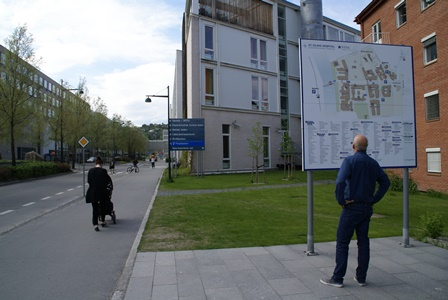
\includegraphics[width=10cm]{figs/findway.jpg}
\caption{A map of St. Olavs Hospital, Trondheim, Norway \cite{stolavs}.}
\label{fig:stolavs}
\end{figure}

Figure \ref{fig:q2} shows the result from Q2: "Are you currently using an indoor map system?" This question was asked in order to gain a sense of the feasibility of churning existing users of indoor map systems to a freemium service. If a respondent responded "yes", then the respondent was of interest of the surveyor due to the possibility of this actor to switch to a indoor map system based on the premises of the freemium model. Conversely, a "no" might indicate a potential first time buyer of an indoor map system. In the case of the latter, factors discussed in Q7 are of interest, as these respondents may have economic constraints or objections that are readily accomodated by offering a freemium product. An overwhelming majority, 78,6\%, responded "no", whereas 21,6\% reported an existing indoor mapping system already in place. This may indicate that the market is unaware of or otherwise disinterested in indoor mapping solutions, something the surveyor intended to remedy in relation to Q7, where respondents were given some potentially beneficiary reasons as to what acquire an indoor mapping system entails.

\begin{figure}
\centering
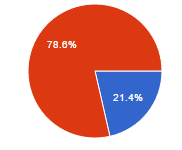
\includegraphics{figs/Q2.PNG}
\caption{Q2: "Are you currently using an indoor map system?". Red indicating "No" and blue indicating "yes"}
\label{fig:q2}
\end{figure}

\section{Potential Acquisition of an Indoor Mapping System - Group 2}
Q3 was asked in order to map the respondent's initial interest and willingness to potentially acquire an indoor mapping system, if no such system was already in place. An even divide of 50\% of "yes" and "no" was the result of asking this particular question. This may indicate indifference between the respondents who replied with "no", but it might also indicate a disinterest in acquiring an indoor mapping system. In hindsight, this question should probably have asked the respondents to specify a reason as to why no such consideration were being made. 
\begin{figure}[H]
\centering
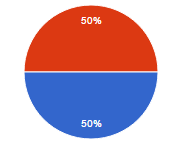
\includegraphics{figs/q3.PNG}
\caption{Q3: "If currently not using an indoor map system, are you considering using an indoor map system?". Red indicating "no" and blue indicating "yes"}
\label{fig:q3}
\end{figure}
To obtain a sense of the respondent's willingness to pay Q4 was asked. As with Q1 this was a qualitative question in nature, and the respondents were given a text input field to submit their answer. A lot of respondents expressed a lot of uncertainty regarding this point, as acquiring and gathering the financial means to put an indoor mapping system into place is not a one-person decision. However, some estimated figures of several NOK $100.000$, based on the inherent intelligence and qualities of the system.
\newline
\\
If potential buyers of indoor mapping solutions are reluctant to acquire such a product, price might be a big factor. In order to gain a sense of how strongly this factor weighs, and potential thoughts around it, Q5 was asked. Several respondents were sceptical and raised concerns regarding quality, stating that "there is no such thing as free". Moreover, long term costs were considered as well citing that capital expenses might be overshadowed by long-running operational costs. 
\newline
\\
Q6: "Would additional, value-adding, paid services on top of a free, basic service be of interest?" were targeted to respondents with the sole purpose of trying to determine whether a freemium model in particular is a feasible economic model. As stated in Chapter 2 - Background, the freemium paradigm requires that the few pays for the many, by purchasing (or otherwise taking use of) a product or a service. As respondents were largely unaware of what these services might include, the answers were mostly negative in nature. In hindsight, a more thorough introduction to what values an indoor mapping solution might add to an establishment, along with potential value added services should have been specified and made clear for the respondents. 
\section{Regarding Disinterest in Indoor Mapping Systems - Group 3}
This group contains one question, namely Q7. As previously stated, Q2 was asked to determine if current users of indoor mapping systems could potentially switch to a freemium service, and Q7 attempted to remedy the disinterested user, by asking respondents what underlying factors that may be the underlying reason as to why an indoor mapping solution was not wanted. At this point in the survey, respondents were made aware of potential benefits that an indoor mapping system may add to their establishment. These included the inherent need users of an establishment have to find a desired location, regardless of size of the establishment. Additionally, a point was made regarding the ever growing Internet-of-things \cite{gilpress2014}, and the need for fleet management \cite{gregsterling2012} in growing businesses. 
\begin{figure}
\centering
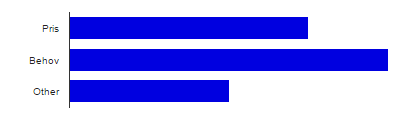
\includegraphics{figs/q7.PNG}
\caption{Q7: "If such a system is not wanted in general terms, which underlying factors decides this?" From top to bottom: "Price", "Demand", "Other"}
\label{fig:my_label}
\end{figure}
Q7 asked respondents to mark any of the applicable options of "price", "demand" and/or "other", where the respondent was given the possibility to specify what "other" might entail. The results were 50\% stating "price", 66,7\% stating "demand" and 33,3\% stated "other". Given the few number of responses, these figures are hardly conclusive, but it may indicates a concern among potential employers of indoor mapping systems, that the demand for the service itself is low. However, given the concerns regarding price of such a system, it might be in favor of a freemium service, if price is seen as a main barrier in acquiring an indoor mapping system. 

\section{Interest For Value-Adding Services - Group 4}
For this group of questions, Q8 was asked, where respondents were asked to decide to what degree they would be interested in paying for a service; a 1 indicating a complete lack of willingness to pay for a service, and 5 indicating a strong willingness to pay for a service. A total of five questions were asked, and they will henceforth be referred to as Q8.1, Q8.2 etc. Statistics from these questions are found in Table \ref{table:gr4}

\begin{figure}[H]
\centering
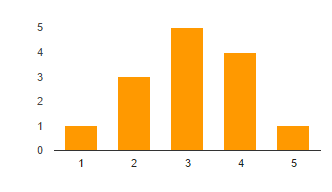
\includegraphics{figs/q81.PNG}
\caption{Q8.1: "Navigation and indoor pathfinding". Vertical axis denotes number of responses.}
\label{fig:q81}
\end{figure}
Figure \ref{fig:q81} shows the result from the first question asked in this group. With a mean of 3,071, standard deviation of 1,072 and the most common answer being "Neutral (3)" not can be concluded from this. Being slightly above the indifference option does not indicate any particular interest for or against paying for indoor navigation. Given the nature of responses given in previous questions, this may not be surprising as a good portion of respondents indicated no desire and lack of motivation for acquiring an indoor mapping solution to begin with. This may also be the case for the rest of the questions asked under Q8, as additional services holds no merit for the buyer should they be disinterested in an indoor mapping system to begin with.

\begin{table}[]
\centering
\begin{tabular}{|l|l|l|l|l|l|}
\hline
\textbf{Parameter} & \textbf{Q8.1} & \textbf{Q8.2}   & \textbf{Q8.3}   & \textbf{Q8.4} & \textbf{Q8.5} \\ \hline
Sample size        & 14            & 14              & 14              & 14            & 14            \\ \hline
Mean               & 3,071         & 3,357           & 3,643           & 3,071         & 2,929         \\ \hline
Mode               & Neutral (3)   & Interesting (4) & Interesting (4) & Neutral (3)   & Neutral (3)   \\ \hline
Standard Deviation & 1,072         & 1,336           & 1,277           & 1,141         & 1,328         \\ \hline
\end{tabular}
\caption{Statistics Group 4}
\label{table:gr4}
\end{table}

\begin{figure}
\centering
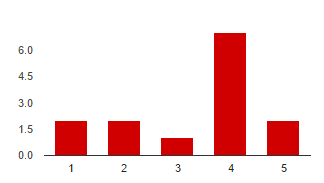
\includegraphics{figs/q82.PNG}
\caption{Q8.2: "Integration with SMS and own apps". Vertical axis denotes number of responses.}
\label{fig:q82}
\end{figure}
Q8.2 along with Q8.5 asked questions regarding the integration with existing systems and infrastructure, however Q8.2 received a more positive response from the respondents: A mean of 3,357, standard deviation of 1,336 and a mode of "Interesting (4)". This indicated that 50\% of respondents were above averagely inclined to pay for an indoor mapping system that integrates with SMS and own apps. These figures might indicate a need to acquire new services on the premises of being integrable with current systems that are not indoor mapping solutions.  
\begin{figure}
\centering
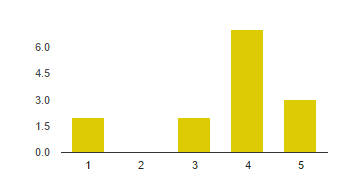
\includegraphics{figs/q83.PNG}
\caption{Q8.3: "Integration with timetables". Vertical axis denotes number of responses}
\label{fig:q83}
\end{figure}
Figure \ref{fig:q83} shows the result of the willingness to pay for a system that integrates with timetables. Naturally, given that the survey was sent out to potential customers of an indoor mapping system with some being airports and shopping malls, the disinterest in this type of additional paid service might be expected to be low to begin with. However, the answers don't reflect this sentiment, as this question garnered the highest mean of the five questions with 3,643. This is also reflected in the most commonly chosen answer "Interesting (4)". This may show an apparent need for integrating an indoor mapping system with a timetable, as is possible at NTNU at the moment: The indoor mapping system MazeMap allows for links to be created which in turn can be embedded into timetables. This allows for integration of an indoor mapping system into timetables \cite{oracleservicentnu}.
\begin{figure}
\centering
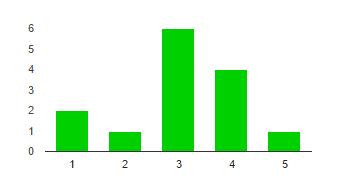
\includegraphics{figs/q84.PNG}
\caption{Q8.4: "Automatic updating of maps". Vertical axis denotes number of responses}
\label{fig:q84}
\end{figure}
Q8.4 asked responders to what degree they would be willing to pay for automatically having their indoor maps updated. This may seem easy enough to grasp in a straightforward manner, however, most of the respondents weren't currently employing an indoor mapping system, and as such they might not be able to see any value in having their indoor maps automatically updated. Thus, it was to be expected that this question would result in a lower score, but it corresponded to a mean of 3,071, the same as Q8.1, with a standard deviation of 1,141 and a mode of "Neutral (3)". 
\begin{figure}
\centering
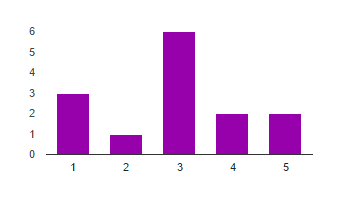
\includegraphics{figs/q85.PNG}
\caption{Q8.5: "Integration of maps into own systems"}
\label{fig:q85}
\end{figure}
Q8.5 (though akin to Q8.2), let the respondents freely decide what they associated with "own systems". This question gathered the lowest mean of the questions with 2,929, a standard deviation of 1,328 and a mode of "Neutral (3)". The low score may indicate privacy concerns of the respondents, but this is only speculation as no qualitative answer or comments from the respondents was possible in relation to questions in Group 4. It could also mean that (as these questions aimed to answer) they were simply not willing to pay for this value-adding service.

\section{More or Less Interest in a Freemium system - Group 5}
The final question, Q9, was a qualitative question where existing owners of indoor mapping systems were asked directly if a free system with the possibility of purchasing value-added services would be more or less interesting than the current system employed. In the context of HEIs and Hospitals in Norway, these are prone to the law public procurements \cite{procurement}, which means that if a public entity wishes to procure a certain service, the type of service has to be announced to the public. Then, a period of time has to pass before any procurement can take place, during which bids are the norm. This is to ensure competition in the market and to hinder corruption. One respondent replied:
\begin{displayquote}
\textit{"We have to deal with the rulings of public procurement, and it would be the total cost that is the underlying factor. The content of the "basic" package is detrimental to a potential procurement, as it may trigger further needs for more services. If a(n) [indoor mapping] system can satisfy the demands and rules of a public procurement, then this is of interest".}
\end{displayquote}
In terms of potential buyers of a freemium service, the public authorities will potentially demand more from the "basic" package, as an overview of total costs is needed. This is harder to determine in this context, as some value-added services might not be deemed necessary in a tryout period.
Some replied simply "no" or "maybe" to this question, but the majority of respondents indicated an interest vague or otherwise more engaged. 